\documentclass[12pt]{article}

\usepackage{tikz} % картинки в tikz
\usepackage{microtype} % свешивание пунктуации
\usepackage{array} % для столбцов фиксированной ширины
\usepackage{comment} % для комментирования целых окружений
\usepackage{indentfirst} % отступ в первом параграфе

\usepackage{sectsty} % для центрирования названий частей
\allsectionsfont{\centering}

\usepackage{amsmath, amssymb, amsthm, amsfonts} % куча стандартных математических плюшек

\usepackage[top=2cm, left=1cm, right=1cm, bottom=2cm]{geometry} % размер текста на странице
\usepackage{lastpage} % чтобы узнать номер последней страницы
 
\usepackage{enumitem} % дополнительные плюшки для списков
%  например \begin{enumerate}[resume] позволяет продолжить нумерацию в новом списке

\usepackage{caption} % подписи к рисункам
\usepackage{hyperref} % гиперссылки
\usepackage{multicol} % текст в несколько столбцов


\usepackage{fancyhdr} % весёлые колонтитулы
\pagestyle{fancy}
\lhead{Введение в глубокое обучение, ЭМИТ, РАНХ}
\chead{}
\rhead{2022-04-27}
\lfoot{Вариант $\zeta$}
\cfoot{Паниковать запрещается!}
% \rfoot{Тест}
\renewcommand{\headrulewidth}{0.4pt}
\renewcommand{\footrulewidth}{0.4pt}

\usepackage{ifthen} % для написания условий

\usepackage{todonotes} % для вставки в документ заметок о том, что осталось сделать
% \todo{Здесь надо коэффициенты исправить}
% \missingfigure{Здесь будет Последний день Помпеи}
% \listoftodos --- печатает все поставленные \todo'шки


% более красивые таблицы
\usepackage{booktabs}
% заповеди из докупентации:
% 1. Не используйте вертикальные линни
% 2. Не используйте двойные линии
% 3. Единицы измерения - в шапку таблицы
% 4. Не сокращайте .1 вместо 0.1
% 5. Повторяющееся значение повторяйте, а не говорите "то же"


\usepackage{fontspec}
\usepackage{polyglossia}

\setmainlanguage{russian}
\setotherlanguages{english}

% download "Linux Libertine" fonts:
% http://www.linuxlibertine.org/index.php?id=91&L=1
\setmainfont{Linux Libertine O} % or Helvetica, Arial, Cambria
% why do we need \newfontfamily:
% http://tex.stackexchange.com/questions/91507/
\newfontfamily{\cyrillicfonttt}{Linux Libertine O}

% Математические шрифты 
\usepackage{unicode-math}     
\setmathfont[math-style=upright]{[Neo Euler.otf]} 

\AddEnumerateCounter{\asbuk}{\russian@alph}{щ} % для списков с русскими буквами
\setlist[enumerate, 2]{label=\asbuk*),ref=\asbuk*}



% мои цвета https://www.artlebedev.ru/colors/
\definecolor{titleblue}{rgb}{0.2,0.4,0.6} 
\definecolor{blue}{rgb}{0.2,0.4,0.6} 
\definecolor{red}{rgb}{1,0,0.2} 
\definecolor{green}{rgb}{0,0.6,0} 
\definecolor{purp}{rgb}{0.4,0,0.8} 

% цвета из geogebra 
\definecolor{litebrown}{rgb}{0.6,0.2,0}
\definecolor{darkbrown}{rgb}{0.75,0.75,0.75}

% Гиперссылки
\usepackage{xcolor}   % разные цвета

\usepackage{hyperref}
\hypersetup{
	unicode=true,           % позволяет использовать юникодные символы
	colorlinks=true,       	% true - цветные ссылки
	urlcolor=blue,          % цвет ссылки на url
	linkcolor=black,          % внутренние ссылки
	citecolor=green,        % на библиографию
	breaklinks              % если ссылка не умещается в одну строку, разбивать её на две части?
}

% эпиграфы
\usepackage{epigraph}
\setlength\epigraphwidth{.6\textwidth}
\setlength\epigraphrule{0pt}

% Математические операторы первой необходимости:
\DeclareMathOperator{\sgn}{sign}
\DeclareMathOperator*{\argmin}{arg\,min}
\DeclareMathOperator*{\argmax}{arg\,max}
\DeclareMathOperator{\Cov}{Cov}
\DeclareMathOperator{\Var}{Var}
\DeclareMathOperator{\Corr}{Corr}
\DeclareMathOperator{\E}{\mathop{E}}
\DeclareMathOperator{\Med}{Med}
\DeclareMathOperator{\Mod}{Mod}
\DeclareMathOperator*{\plim}{plim}

\DeclareMathOperator{\logloss}{logloss}
\DeclareMathOperator{\softmax}{softmax}

\DeclareMathOperator{\tr}{tr}

% команды пореже
\newcommand{\const}{\mathrm{const}}  % const прямым начертанием
\newcommand{\iid}{\sim i.\,i.\,d.}  % ну вы поняли...
\newcommand{\fr}[2]{\ensuremath{^{#1}/_{#2}}}   % особая дробь
\newcommand{\ind}[1]{\mathbbm{1}_{\{#1\}}} % Индикатор события
\newcommand{\dx}[1]{\,\mathrm{d}#1} % для интеграла: маленький отступ и прямая d

% одеваем шапки на частые штуки
\def \hb{\hat{\beta}}
\def \hs{\hat{s}}
\def \hy{\hat{y}}
\def \hY{\hat{Y}}
\def \he{\hat{\varepsilon}}
\def \hVar{\widehat{\Var}}
\def \hCorr{\widehat{\Corr}}
\def \hCov{\widehat{\Cov}}

% Греческие буквы
\def \a{\alpha}
\def \b{\beta}
\def \t{\tau}
\def \dt{\delta}
\def \e{\varepsilon}
\def \ga{\gamma}
\def \kp{\varkappa}
\def \la{\lambda}
\def \sg{\sigma}
\def \tt{\theta}
\def \Dt{\Delta}
\def \La{\Lambda}
\def \Sg{\Sigma}
\def \Tt{\Theta}
\def \Om{\Omega}
\def \om{\omega}

% Готика
\def \mA{\mathcal{A}}
\def \mB{\mathcal{B}}
\def \mC{\mathcal{C}}
\def \mE{\mathcal{E}}
\def \mF{\mathcal{F}}
\def \mH{\mathcal{H}}
\def \mL{\mathcal{L}}
\def \mN{\mathcal{N}}
\def \mU{\mathcal{U}}
\def \mV{\mathcal{V}}
\def \mW{\mathcal{W}}

% Жирные буквы
\def \mbb{\mathbb}
\def \RR{\mbb R}
\def \NN{\mbb N}
\def \ZZ{\mbb Z}
\def \PP{\mbb{P}}
\def \QQ{\mbb Q}

\def \putyourname{\fbox{
    \begin{minipage}{42em}
      Фамилия, имя, номер группы:\vspace*{3ex}\par
      \noindent\dotfill\vspace{2mm}
    \end{minipage}
  }
}

\def \checktable{

	\vspace{5pt}
	Табличка для проверяющих работу:

\vspace{5pt}

	\begin{tabular}{|m{2cm}|m{1cm}|m{1cm}|m{1cm}|m{1cm}|m{1cm}|m{2cm}|}
\toprule
		Тест & 1 &  2 & 3 & 4 & 5 & Итого \\
\midrule
		&  &  & & & & \\
		&  &  & & & & \\
 \bottomrule
\end{tabular}
}


\def \testtable{

\vspace{5pt}
	Внесите сюда ответы на тест:

\vspace{5pt}

\begin{tabular}{|m{2cm}|m{0.6cm}|m{0.6cm}|m{0.6cm}|m{0.6cm}|m{0.6cm}|m{0.6cm}|m{0.6cm}|m{0.6cm}|m{0.6cm}|m{0.6cm}|}
\toprule
		Вопрос & 1 &  2 & 3 & 4 & 5 & 6 & 7 & 8 & 9 & 10 \\
\midrule
		Ответ &  &  & & & & & & & & \\
 \bottomrule
\end{tabular}
}


% [1][3] 1 = one argument, 3 = value if missing
% эта магия создаёт окружение answerlist
% именно в окружении answerlist записаны варианты ответов в подключаемых exerciseXX
% просто \begin{answerlist} сделает ответы в три столбца
% если ответы длинные, то надо в них руками сделать
% \begin{answerlist}[1] чтобы они шли в один столбец
\newenvironment{answerlist}[1][3]{
\begin{multicols}{#1}

\begin{enumerate}[label=\fbox{\emph{\Alph*}},ref=\emph{\alph*}]
}
{
\item Нет верного ответа.
\end{enumerate}
\end{multicols}
}

% BB: unicol version. don't know why \ifthenelse fails in second part of new-env
\newenvironment{answerlistu}{
\begin{enumerate}[label=\fbox{\emph{\Alph*}},ref=\emph{\alph*}]
}
{
\item Нет верного ответа.
\end{enumerate}
}


\excludecomment{solution} % without solutions

\theoremstyle{definition}
\newtheorem{question}{Вопрос}

\usepackage{tikzlings}
\usepackage{tikzducks}

\usepackage{alltt}

\begin{document}

\putyourname

% \testtable

% \checktable

\epigraph{\textit{(Профессор Фарнсворт, наблюдая в телескоп, как Фрай и Лила убегают с темной стороны Луны):} \\ \mbox{ } \\ Бог мой! Надо бы что-то предпринять... Но я уже в пижаме... \\ \mbox{ } \\ \textit{(Фарнсворт засыпает на стуле)}}{\textit{Футурама (1999)}}


Работа состоит из трёх частей: тестовая, задачи и ответы на открытые вопросы. Списывание карается обнулением работы. Ко всем одинаковым формулировкам я буду очень сильно придираться. Удачи!


\section*{Часть первая: тестовая} 

Дайте ответ на $10$ тестовых вопросов. Каждый вопрос стоит $3$ балла. Никакие дополнительные пояснений в этой части работы от вас не требуются.

\begin{question}
Что из этого формула для шага в градиентном спуске? 
\begin{answerlist}
  \item \(w_t = w_{t-1} - \eta \cdot \nabla L(w_{t})\) 
  \item \(w_t = w_{t-1} + \eta \cdot \nabla L(w_{t})\)
  \item \(w_t = w_{t-1} - \eta \cdot \nabla L(w_{t-1})\)
  \item \(w_t = w_{t-1} - \eta \cdot \nabla L(w_{0})\)
  \item \(w_t = w_{t-1} + \eta \cdot \nabla L(w_{t-1})\) 
\end{answerlist}
\end{question}

\begin{solution}
\begin{answerlist}
  \item Bad answer :(
  \item Bad answer :(
  \item Good answer :)
  \item Bad answer :(
  \item Bad answer :(
\end{answerlist}
\end{solution}


\begin{question}
Какие из следующих функций активации подходят для обучения нейронных сетей?
\begin{answerlist}
  \item \(f(z) = \max(0.25z, 0.75z) \)
  \item \(f(z) = \min(0, z) \)
  \item \(f(z) = 0.25 z \)
  \item \(f(z) = \begin{cases} 1, x > 0.5 \\ -1, x \le 0.5 \end{cases} \)
  \item \(f(z) = 1 - z \)
\end{answerlist}
\end{question}

\begin{solution}
\begin{answerlist}
  \item Good answer :)
  \item Good answer :)
  \item Bad answer :(
  \item Bad answer :(
  \item Bad answer :(
\end{answerlist}
\end{solution}

\begin{question}
Яродар берёт картинку и пририсовывает ей с каждой стороны четыре дополнительные клетки. Свёртка какого размера не изменит размер исходной картинки?  % 9 x 9
\begin{answerlist}
  \item \(3 \times 3\)
  \item \(4 \times 4\)
  \item \(5 \times 5\)
  \item \(6 \times 6\)
  \item \(7 \times 7\)
\end{answerlist}
\end{question}

\begin{solution}
\begin{answerlist}
  \item Bad answer :(
  \item Bad answer :(
  \item Bad answer :(
  \item Bad answer :(
  \item Bad answer :(
\end{answerlist}
\end{solution}

\begin{question}
Какие из следующих техник можно использовать, чтобы избежать переобучения? 
\begin{answerlist}
  \item Аугментация данных (Data augmentation)
  \item Нормализация по батчам (Batch Normalization)
  \item Использовать Adam вместо SGD
  \item Ранняя остановка обучения (Early stopping)
  \item Дропаут (Dropout)
\end{answerlist}
\end{question}

\begin{solution}
\begin{answerlist}
  \item Good answer :)
  \item Good answer :)
  \item Bad answer :(
  \item Good answer :)
  \item Good answer :)
\end{answerlist}
\end{solution}

\newpage 

\begin{question}
После обучения нейронной сети, вы обнаружили, что accuracy на тренировочной выборки равен $100\%,$  а accuracy на тестовой выборке равен $42\%$. Какие из следующих методов могут помочь сократить разницу между этими двумя метриками? 
\begin{answerlist}
  \item Сигмоида в качестве активации
  \item Dropout
  \item Алгоритм обратного распространения ошибки
  \item Softmax
  \item RMSprop
\end{answerlist}
\end{question}

\begin{solution}
\begin{answerlist}
  \item Bad answer :(
  \item Good answer :)
  \item Bad answer :(
  \item Bad answer :(
  \item Bad answer :(
\end{answerlist}
\end{solution}


\begin{question}
Выберите все верные утверждения 
\begin{answerlist}
  \item Если мы используем сигмоиду в качестве функции активации, при обратном проходе через неё производная никогда не поменяет знак
  \item Картинки нормируют на отрезок $[-1; 1]$ для более быстрой сходимости обучения
  \item Если мы используем Leaky ReLU в качестве функции активации, при обратном проходе через неё производная никогда не поменяет знак
  \item Картинки нормируют на отрезок $[0; 1]$ для более быстрой сходимости обучения
  \item В нормализации по батчам нет параметров, которые можно было бы обучить алгоритмом обратного распространения ошибки
\end{answerlist}
\end{question}

\begin{solution}
\begin{answerlist}
  \item Good answer :)
  \item Good answer :)
  \item Bad answer :(
  \item Bad answer :(
  \item Bad answer :(
\end{answerlist}
\end{solution}


\begin{question}
Выберите все верные утверждения об инициализации Хе
\begin{answerlist}
  \item Такая инициализация используется только в полносвязных сетях.
  \item Такая инициализация используется только в свёрточных сетях.
  \item Такая инициализация используется для симметричных функций активации вроде сигмоиды
  \item Такая инициализация используется для функций активации вроде ReLU
  \item Инициализация Хе корректируют параметры распределений в зависимости от входа и выхода слоя так, чтобы поддерживать дисперсию равной единице
\end{answerlist}
\end{question}

\begin{solution}
\begin{answerlist}
  \item Bad answer :(
  \item Bad answer :(
  \item Bad answer :(
  \item Good answer :)
  \item Good answer :)
\end{answerlist}
\end{solution}


\begin{question}
У нас есть $10$ классов. Классификатор предсказывает, что объект равновероятно относится к каждому из них. Какое значение принимает logloss на этом объекте? 
\begin{answerlist}
  \item \(-\log 10 \)
  \item \(-0.1 \log 1 \)
  \item \(-\log 0.1 \)
  \item \(-10 \log 0.1 \)
  \item \(-10 \log 10 \)
\end{answerlist}
\end{question}

\begin{solution}
\begin{answerlist}
  \item Bad answer :(
  \item Bad answer :(
  \item Good answer :)
  \item Bad answer :(
  \item Bad answer :(
\end{answerlist}
\end{solution}


\begin{question}
К изображению размера $W \times H$ применили $D$ фильтров. Получилось новое изображение размера $W \times H \times D$. К немы мы хотим применить свёртку размера $1 \times 1.$ Сколько параметров нам надо будет обучить в этой свёртке? 
\begin{answerlist}
  \item  $1$
  \item  $W \cdot H$
  \item  $D$
  \item  $W$
  \item  $H$
\end{answerlist}
\end{question}

\begin{solution}
\begin{answerlist}
  \item Bad answer :(
  \item Bad answer :(
  \item Good answer :)
  \item Bad answer :(
  \item Bad answer :(
\end{answerlist}
\end{solution}

\newpage 

\begin{question}
Выберите функции, которые могли бы описать части вычислительного графа, представленного ниже. Рёбрам соответствуют какие-то веса, а вершинам любые алгебраические операции и применения основных элементарных функций (экспонента, косинус и тп).

    \begin{center}
    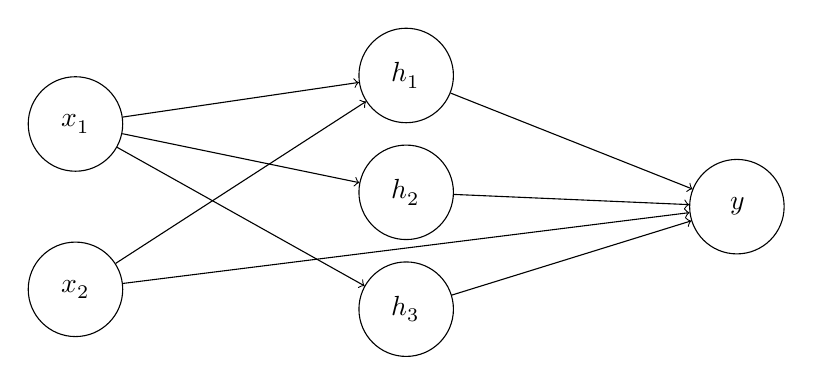
\begin{tikzpicture}[scale=1.4]
    	\tikzstyle{place}=[circle, draw=black, minimum size = 12mm]
    	\tikzstyle{placeh}=[draw=black, minimum height=25pt,minimum width=60pt,inner sep=2pt]
    	
    	% Input
    	\foreach \x in {1,...,2}
    	\draw node at (0, -\x*1.5) [place] (first_\x) {$x_\x$};
    	
    	% Hidden 1
    	\foreach \x in {1,...,3}
    	\node at (3, -\x*1.06) [place] (second_\x){$h_\x$};		
    	
    	% Output
    	\node at (6, -2.25) [place] (fourth){$y$};
    	
    	\draw [->]  (first_1) to (second_1);
    	\draw [->]  (first_1) to (second_2);
    	\draw [->]  (first_1) to (second_3);
    	\draw [->]  (first_2) to (second_1);
    	
    	\draw [->]  (second_1) to (fourth);
    	\draw [->]  (second_2) to (fourth);
    	\draw [->]  (second_3) to (fourth);
    	
    	\draw [->]  (first_2) to (fourth);

    \end{tikzpicture}
    \end{center} 

\begin{answerlist}
  \item  $h_1 = x_1^2 + x_2$
  \item  $h_2 = e^{x_1}$
  \item  $h_3 = 2 x_1 + 3 x_2$
  \item  $y = 2h_1 + 3 h_2 + h_3$
  \item  $h_3 = 2 x_1$
\end{answerlist}
\end{question}

\begin{solution}
\begin{answerlist}
  \item Bad answer :(
  \item Good answer :)
  \item Bad answer :(
  \item Good answer :)
  \item Good answer :)
\end{answerlist}
\end{solution}

\newpage 

 
\section*{Часть вторая: задачки}

Все ответы должны быть обоснованы. Решения должны быть прописаны для каждого пункта. Рисунки должны быть чёткими и понятными. Все линии должны быть подписаны. За решение каждой задачи можно получить 8 баллов.

\begin{question}
    Рассмотрим следующие две функции активации: сигмоиду и гиперболический тангенс 
    
    \[
    \sigma(z) = \frac{1}{1 + e^{-z}} \qquad \tanh(z) = \frac{e^z - e^{-z}}{e^z + e^{-z}}.
    \]
    
    \begin{enumerate}
    \item Как взаимосвязаны $\sigma(z)$ и $\sigma'(z)$?  Как взаимосвязаны $\tanh(z)$ и $\tanh'(z)$? 
    \item Выпишите уравнения для шага обратного распространения для обеих функций активации. 
    \item Что такое паралич нейронной сети? Как сигмоида способствует ему? Способствует ли параличу гиперболический тангентс? 
    \item Объясните, почему использование гиперболического тангентса вместо сигмоиды делает оптимизацию нейронной сети проще. Какие проблемы использование тангентса не исправляет?
    \end{enumerate} 
\end{question}


\newpage 

\begin{question}
Предположим, что у вас есть цветная картинка размера $10 \times 10 \times 3$. Вы хотите собрать сетку из двух свёрточных слоёв с ядром размера $3 \times 3$ с $10$ и $20$ фильтрами. Сколько параметров нужно будет оценить в этих двух слоях? Не забудьте про константу! 
\end{question}

\vspace{8cm} 

\begin{question}
Мы обучаем нейронную сеть из $N$ свёрточных слоёв размера $k \times k$ с параметром сдвига (stride) равным единице. Дополнение картинки (padding) не делается. Нумерация слоёв начинается с единицы. Выпишите формулу, по которой можно вычислить размер поля обзора (receptive field) сети.
\end{question}


\newpage 

\begin{question}
Решите следующую задачу матричной оптимизации. Убедитесь, что найденное решение действительно является минимумом. 

\[
f(x) = x^T A x - x^Tb + c \to \min_{x}
\]
\end{question}

\vspace{6cm} 

\begin{question}
Предположим, что softmax принимает на вход вектор $z_1, \ldots, z_k$ и возвращает вектор $p_1, \ldots p_k$. Мы можем записать функцию в виде двух уравнений

\[
r = \sum_{j = 1}^k e^{z_j} \qquad y_i = \frac{e^{z_i}}{r}.
\]

\begin{enumerate} 
    \item Пусть $k=3$. Нарисуйте граф вычислений, на котором описывается взаимосвязь между величинами $z_1, z_2, z_3, p_1, p_2, p_3$ и $r$. 
    
    \item Опишите алгоритм обратного распространения ошибки для softmax-слоя. Выпишите формулу, по которой обновляется градиент при проходе через softmax. 
\end{enumerate} 
\end{question}


\newpage 


\section*{Часть третья: открытые вопросы}

Эта часть состоит из открытых вопросов. На них необходимо дать краткие, но ёмкие ответы. За ответ на каждый вопрос можно получить 5 баллов.


\begin{question}
    Есть теорема, которая говорит, что двухслойной нейронной сетью можно приблизить любую непрерывную функцию. Почему люди не ограничиваются двумя слоями и учат глубокие нейронные сети? 
\end{question}

\vspace{8cm} 

\begin{question}
   Можно ли утверждать, что оптимизация градиентным спуском гарантирует нахождение глобального оптимума весов глубокой нейронной сети?  Почему?
\end{question}

\newpage 

\begin{question}
    Объясните, почему инициализировать в нейронной сети веса константами --- плохая идея?
\end{question}


\vspace{8cm} 


\begin{question}
    Представим себе, что вы реализовали глубокую нейросеть и отправили её учиться. Прошло несколько дней. По логам обучения вы поняли, что нейросеть не хочет учиться. Её качество оказалось лучше случайного, но сильно хуже, чем ожидается в вашей задаче. Какие именно действия вы предпримите, чтобы понять, где именно у вас возникли проблемы?
\end{question}

% % Посмотреть на несколько случайных батчей. Типичные косяки для картинок - нормализация, для текстов - неверная токенизация. Проверить, что данные перемешаны. 
% % Проверить, что сеть может переобучиться на маленькой выборке. 
% % Померить нормы градиентов по всем слоям во время обучения. Косяки: затухание ближе к началу сети, совсем нулевые нормы, взрывы время от времени
% % Посмотреть на кривые обучения. На них можно обнаружить взрывы градиентов, неперемешанные данные, переобучение
% % Показать сеть коллеге за шоколадку 
% % Упростить модель, проверить каждый блок по отдельности 

% % Число мёртвых нейронов по слоям (RELU нейрон мертв если выдает нули на всех примерах)
% % Если фреймворк позволяет накосячить с подсчётом градиентов - надо сравнить их с численными 
% % Много вещей для узкой специфики: использование fp16, распределенность, хитрые задачи вроде RL

\newpage 

\begin{question} 
Однажды на следующий день после жёсткой вечеринки в середине недели ваш коллега написал такую архитектуру нейросети. Она решает задачу классификации RGB-изображения  размера $100 \times 100$ на $10$ классов. Каждое изображение принадлежит только к одному классу. Какие проблемы есть у этой нейросети? 

\begin{alltt}
        model = Sequential() 
        model.add(InputLayer([100, 100, 3]))
        
        model.add(Conv2D(filters=512, kernel\_size=(3, 3), kernel\_initializer="glorot_uniform")) 
        model.add(Activation('relu'))
        model.add(MaxPool2D(pool_size=(2, 2)))
        
        model.add(Conv2D(filters=128, kernel\_size=(3, 3), kernel\_initializer="glorot_uniform")) 
        model.add(Activation('relu'))
        
        model.add(Conv2D(filters=32, kernel\_size=(3, 3), kernel\_initializer="glorot_uniform"))
        model.add(Conv2D(filters=32, kernel\_size=(1, 1), kernel\_initializer="glorot_uniform"))
        model.add(MaxPool2D(pool_size=(10, 10)))
        
        model.add(Flatten()) # convert 3d tensor to a vector of features
        model.add(Dense(64))
        model.add(Dropout(rate=1))
        model.add(Dense(10))
        model.add(Activation('sigmoid'))
        model.add(Dropout(rate=0.5))
\end{alltt}
\end{question}

% % неправильная инициализация для релу
% % дропаут на вероятности в самом конце - сломает функцию потерь и будет мешать обучаться хоть чему-то
% % дропаут 1 - жесть
% % нет активации между линейными слоями

% % инициализация нулями - сеть не будет обучаться из-за эффекта симметрии.
% % -- вариант - кандидат может заметить, что инициализация нулями слоёв с ReLU может привести к тому, что градиенты всю жизнь будут нулевыми
% % инициализация стандартным нормальным распределением может раздуть/уменьшить дисперсию, лучше glorot/xavier/kaiming normal/uniform

% % активация softmax в промежуточном слое - из всего слоя значимо ненулевые значения будут иметь 1-2 нейрона
% % активация sigmoid на последнем слое - в принципе можно (и учить бинарной кроссэнтропией на 1-hot вектор ответа), но для классификации с 1 правильным ответом лучше softmax.
% % свёртка 1x1 - вообще она имеет смысл, но в коде перед ней нет нелинейности, поэтому это лишнее линейное преобразование
% % 512 фильтров размера 3x3 в первом слое - очень много. Как правило, для квадрата 3x3 пикселя кодируются 32-64 фильтров
% % уменьшение числа фильтров вглубь по сети - не очень эффективно, сеть "теряет capacity" - последующие слои могут не уместить всю полезную информацию из предыдущих. Лучше начать с малого и увеличивать.
% % фильтры 10x10 - огромный размер, начиная с какого-то слоя у нас изображение станет меньеш размера фильтра. Да и в целом это неэффективно.
% % max pool 6x6 - очень субъективно, но там где он стоит этот пулинг выбрасывает слишком много информации
% % не ошибка, но можно несколько оптимизировать вычисления, если переставить ReLU после Max Pooling, а результат будет эквивалентный.

\newpage 

\begin{question}
Объясните мем
\begin{center}
	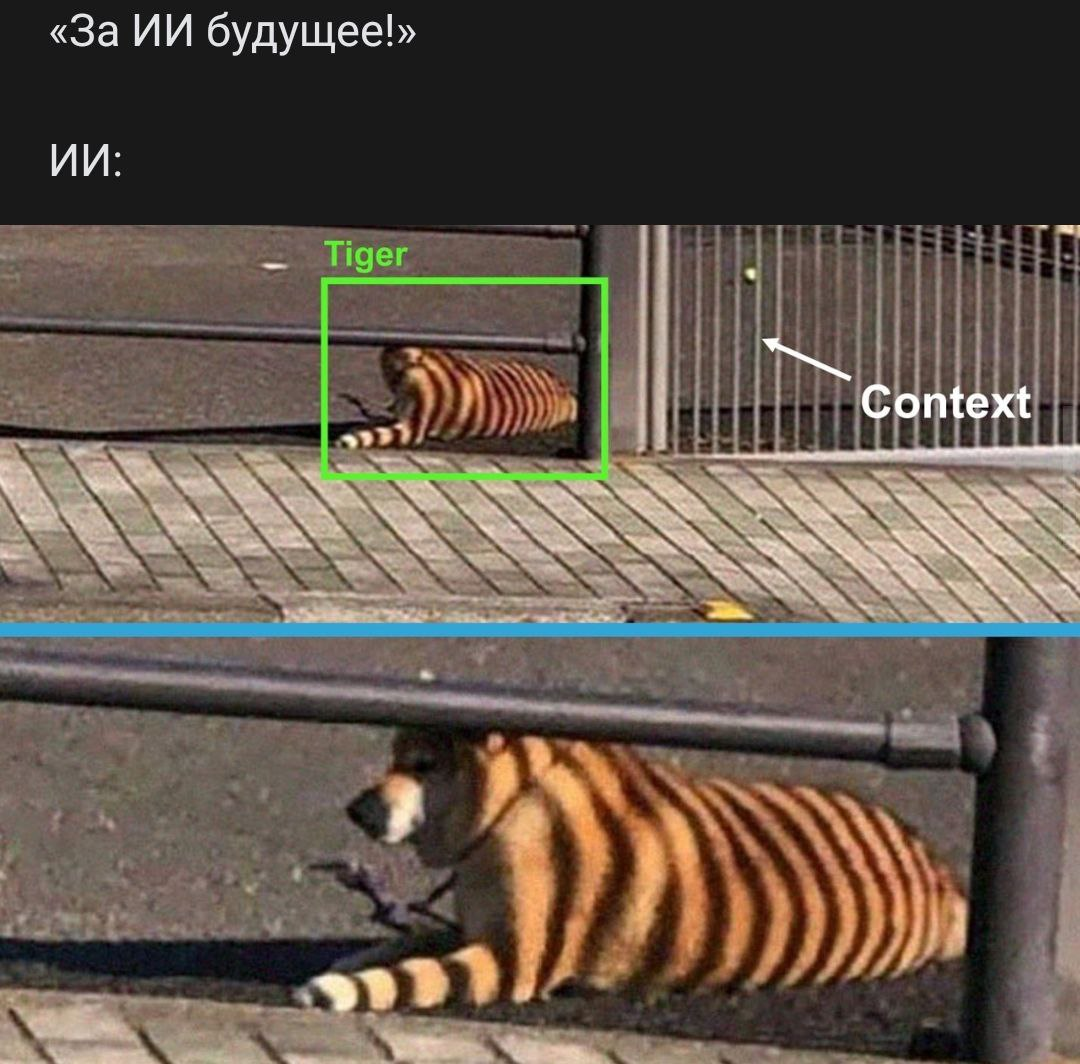
\includegraphics[scale=0.25]{memes_dog.png}
\end{center}
\end{question}

\end{document}
